\documentclass{standalone}
\usepackage{tikz}
\usetikzlibrary{patterns, positioning}
\usepackage[sfdefault]{ClearSans} %% option 'sfdefault' activates Clear Sans as the default text font
\usepackage[T1]{fontenc}

\begin{document}
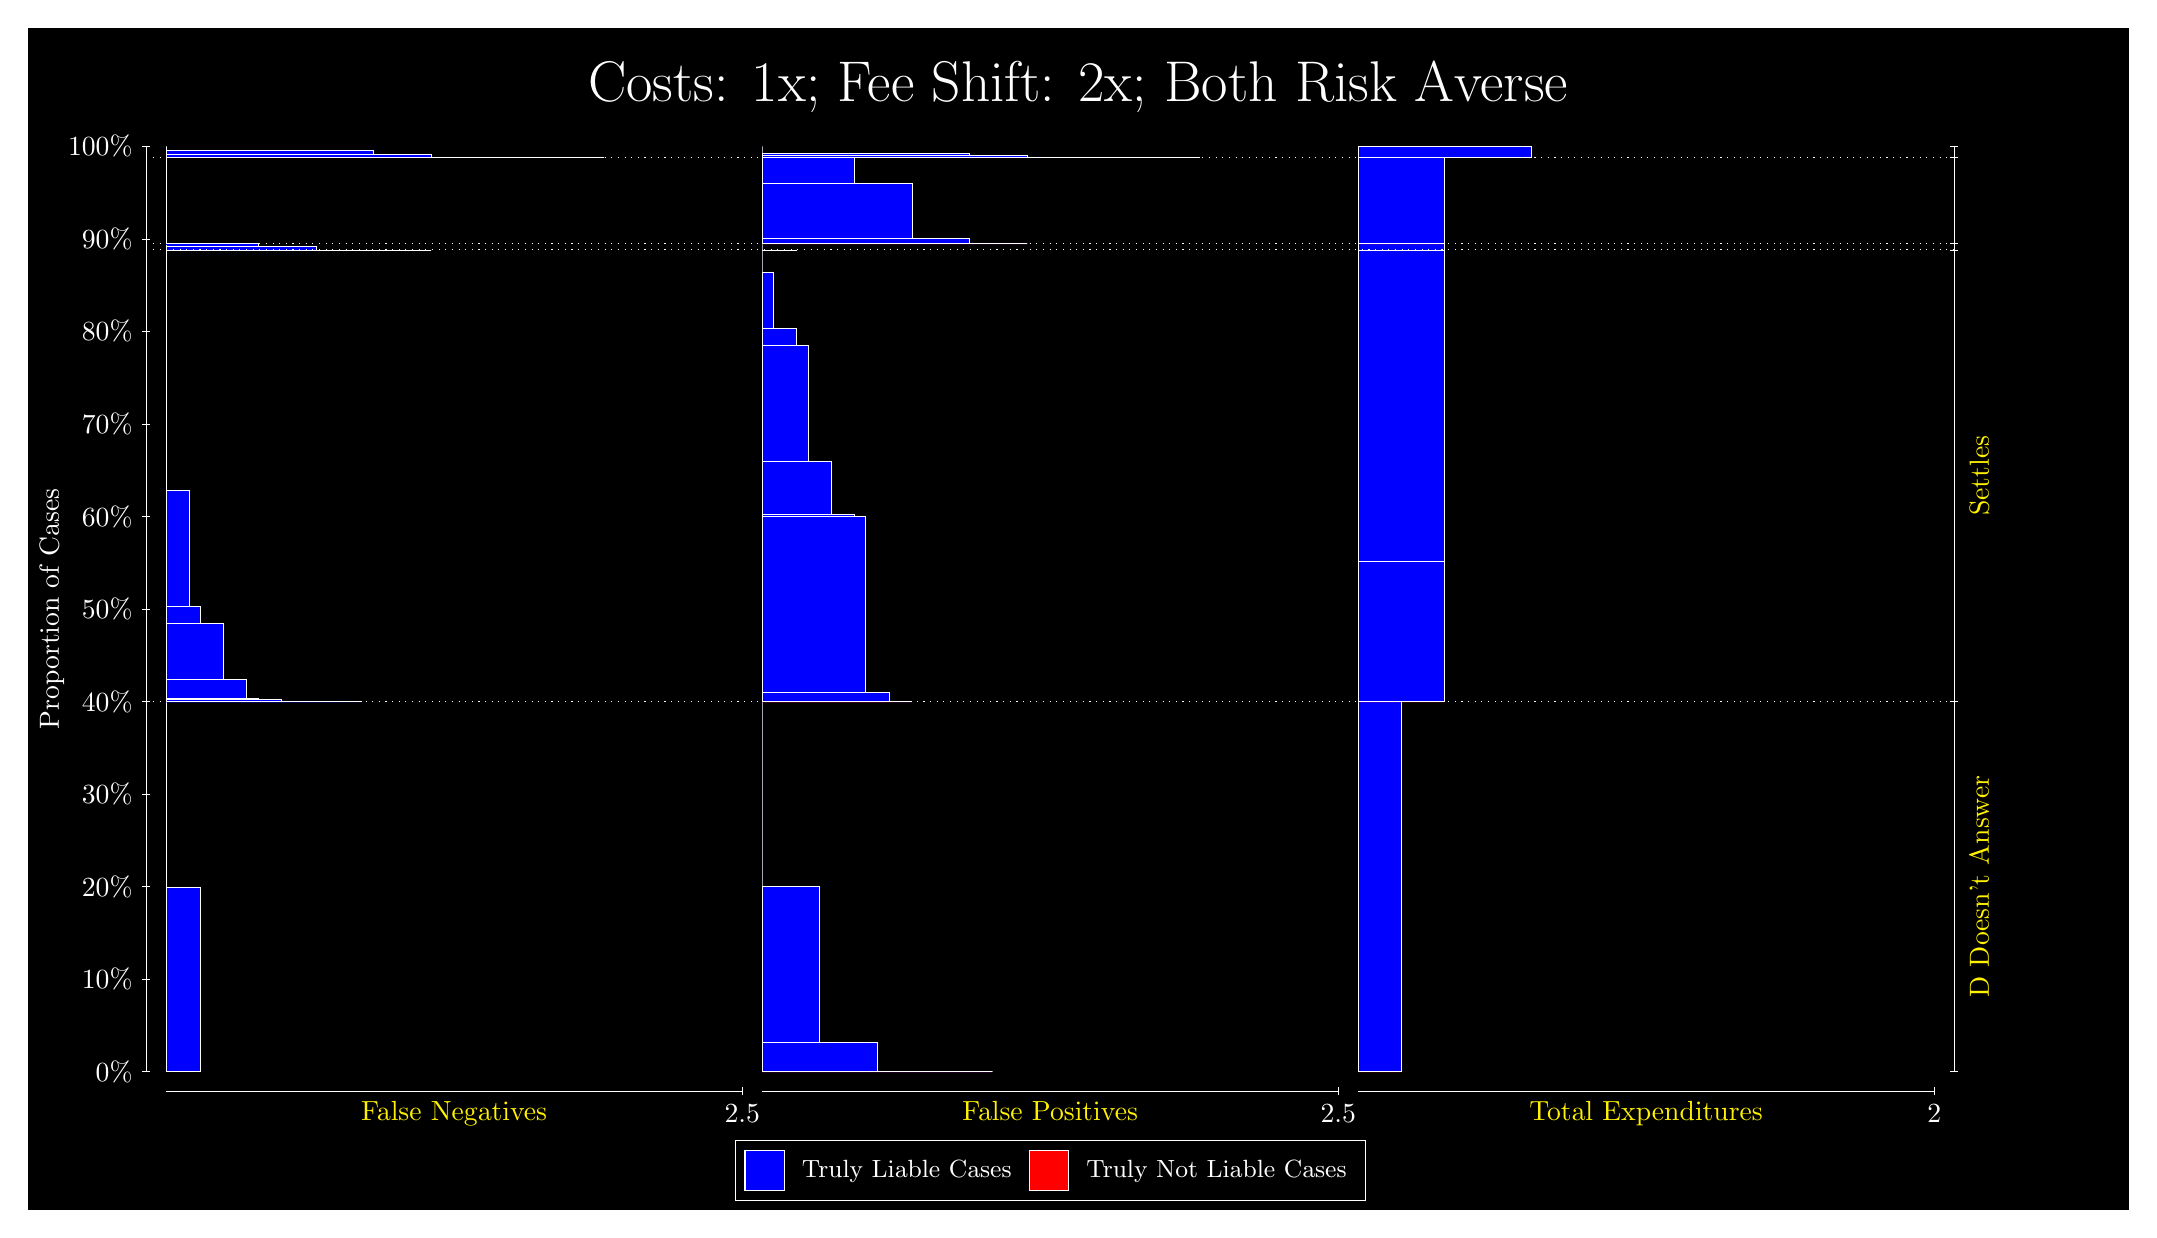
\begin{tikzpicture}
\draw[fill=black] (0,0) rectangle (26.667,15);
\draw[text=white] (0,13.5) rectangle (26.667,15) node[midway] {\huge Costs: 1x; Fee Shift: 2x; Both Risk Averse};
\draw[white, very thin] (1.5,1.75) -- (1.5,13.5);
\node[rotate=90, text=white, anchor=center] at (0.3, 7.625) {Proportion of Cases};
\draw[white, very thin] (1.45,1.75) -- (1.55,1.75);
\node[text=white, anchor=east] at (1.45, 1.75) {0\%};
\draw[white, very thin] (1.45,2.925) -- (1.55,2.925);
\node[text=white, anchor=east] at (1.45, 2.925) {10\%};
\draw[white, very thin] (1.45,4.1) -- (1.55,4.1);
\node[text=white, anchor=east] at (1.45, 4.1) {20\%};
\draw[white, very thin] (1.45,5.275) -- (1.55,5.275);
\node[text=white, anchor=east] at (1.45, 5.275) {30\%};
\draw[white, very thin] (1.45,6.45) -- (1.55,6.45);
\node[text=white, anchor=east] at (1.45, 6.45) {40\%};
\draw[white, very thin] (1.45,7.625) -- (1.55,7.625);
\node[text=white, anchor=east] at (1.45, 7.625) {50\%};
\draw[white, very thin] (1.45,8.8) -- (1.55,8.8);
\node[text=white, anchor=east] at (1.45, 8.8) {60\%};
\draw[white, very thin] (1.45,9.975) -- (1.55,9.975);
\node[text=white, anchor=east] at (1.45, 9.975) {70\%};
\draw[white, very thin] (1.45,11.15) -- (1.55,11.15);
\node[text=white, anchor=east] at (1.45, 11.15) {80\%};
\draw[white, very thin] (1.45,12.325) -- (1.55,12.325);
\node[text=white, anchor=east] at (1.45, 12.325) {90\%};
\draw[white, very thin] (1.45,13.5) -- (1.55,13.5);
\node[text=white, anchor=east] at (1.45, 13.5) {100\%};

\draw[white, very thin] (24.457,1.75) -- (24.457,13.5);
\draw[white, very thin] (24.407,1.75) -- (24.507,1.75);
\node[anchor=west] at (24.407, 1.75) {};
\draw[white, very thin] (24.407,6.4489) -- (24.507,6.4489);
\node[anchor=west] at (24.407, 6.4489) {};
\draw[white, very thin] (24.407,12.185) -- (24.507,12.185);
\node[anchor=west] at (24.407, 12.185) {};
\draw[white, very thin] (24.407,12.264) -- (24.507,12.264);
\node[anchor=west] at (24.407, 12.264) {};
\draw[white, very thin] (24.407,13.361) -- (24.507,13.361);
\node[anchor=west] at (24.407, 13.361) {};
\draw[white, very thin] (24.407,13.5) -- (24.507,13.5);
\node[anchor=west] at (24.407, 13.5) {};

\draw[white, very thin, fill=blue] (1.75,1.75) rectangle (2.1891,4.0962);
\draw[white, very thin, fill=red] (1.75,4.0962) rectangle (1.75,4.0962);
\draw[white, very thin, fill=blue] (1.75,4.0962) rectangle (1.75,6.4489);
\draw[white, very thin, fill=blue] (1.75,6.4489) rectangle (4.2384,6.4489);
\draw[white, very thin, fill=blue] (1.75,6.4489) rectangle (3.9457,6.4489);
\draw[white, very thin, fill=blue] (1.75,6.4489) rectangle (3.6529,6.4489);
\draw[white, very thin, fill=blue] (1.75,6.4489) rectangle (3.5065,6.453);
\draw[white, very thin, fill=blue] (1.75,6.453) rectangle (3.2138,6.4774);
\draw[white, very thin, fill=blue] (1.75,6.4774) rectangle (2.921,6.4882);
\draw[white, very thin, fill=blue] (1.75,6.4882) rectangle (2.7746,6.7308);
\draw[white, very thin, fill=blue] (1.75,6.7308) rectangle (2.4819,7.4442);
\draw[white, very thin, fill=blue] (1.75,7.4442) rectangle (2.1891,7.6619);
\draw[white, very thin, fill=blue] (1.75,7.6619) rectangle (2.0428,9.135);
\draw[white, very thin, fill=red] (1.75,9.135) rectangle (1.75,9.135);
\draw[white, very thin, fill=blue] (1.75,9.135) rectangle (1.75,12.185);
\draw[white, very thin, fill=blue] (1.75,12.185) rectangle (5.1167,12.185);
\draw[white, very thin, fill=blue] (1.75,12.185) rectangle (4.3848,12.186);
\draw[white, very thin, fill=blue] (1.75,12.186) rectangle (3.6529,12.226);
\draw[white, very thin, fill=blue] (1.75,12.226) rectangle (2.921,12.263);
\draw[white, very thin, fill=blue] (1.75,12.263) rectangle (2.1891,12.264);
\draw[white, very thin, fill=red] (1.75,12.264) rectangle (1.75,12.264);
\draw[white, very thin, fill=blue] (1.75,12.264) rectangle (2.1891,12.268);
\draw[white, very thin, fill=red] (1.75,12.268) rectangle (1.75,12.268);
\draw[white, very thin, fill=blue] (1.75,12.268) rectangle (1.75,13.361);
\draw[white, very thin, fill=blue] (1.75,13.361) rectangle (7.3123,13.361);
\draw[white, very thin, fill=blue] (1.75,13.361) rectangle (6.5805,13.361);
\draw[white, very thin, fill=blue] (1.75,13.361) rectangle (5.8486,13.363);
\draw[white, very thin, fill=blue] (1.75,13.363) rectangle (5.1167,13.395);
\draw[white, very thin, fill=blue] (1.75,13.395) rectangle (4.3848,13.445);
\draw[white, very thin, fill=blue] (1.75,13.445) rectangle (3.6529,13.45);
\draw[white, very thin, fill=blue] (1.75,13.45) rectangle (2.921,13.45);
\draw[white, very thin, fill=blue] (1.75,13.45) rectangle (2.3355,13.45);
\draw[white, very thin, fill=red] (1.75,13.45) rectangle (1.75,13.45);
\draw[white, very thin, fill=blue] (1.75,13.45) rectangle (1.75,13.5);
\draw[white, very thin, fill=red] (9.3189,1.75) rectangle (12.246,1.75);
\draw[white, very thin, fill=blue] (9.3189,1.75) rectangle (12.246,1.75);
\draw[white, very thin, fill=blue] (9.3189,1.75) rectangle (11.515,1.7532);
\draw[white, very thin, fill=blue] (9.3189,1.7532) rectangle (10.783,2.126);
\draw[white, very thin, fill=blue] (9.3189,2.126) rectangle (10.051,4.1027);
\draw[white, very thin, fill=blue] (9.3189,4.1027) rectangle (9.3189,6.4489);
\draw[white, very thin, fill=red] (9.3189,6.4489) rectangle (11.222,6.4489);
\draw[white, very thin, fill=blue] (9.3189,6.4489) rectangle (11.222,6.4489);
\draw[white, very thin, fill=red] (9.3189,6.4489) rectangle (10.929,6.4489);
\draw[white, very thin, fill=blue] (9.3189,6.4489) rectangle (10.929,6.5671);
\draw[white, very thin, fill=red] (9.3189,6.5671) rectangle (10.636,6.5671);
\draw[white, very thin, fill=blue] (9.3189,6.5671) rectangle (10.636,8.7969);
\draw[white, very thin, fill=blue] (9.3189,8.7969) rectangle (10.49,8.8221);
\draw[white, very thin, fill=blue] (9.3189,8.8221) rectangle (10.197,9.4989);
\draw[white, very thin, fill=blue] (9.3189,9.4989) rectangle (9.9044,10.972);
\draw[white, very thin, fill=blue] (9.3189,10.972) rectangle (9.758,11.19);
\draw[white, very thin, fill=blue] (9.3189,11.19) rectangle (9.4652,11.903);
\draw[white, very thin, fill=blue] (9.3189,11.903) rectangle (9.3189,12.185);
\draw[white, very thin, fill=red] (9.3189,12.185) rectangle (9.758,12.185);
\draw[white, very thin, fill=blue] (9.3189,12.185) rectangle (9.758,12.186);
\draw[white, very thin, fill=blue] (9.3189,12.186) rectangle (9.3189,12.264);
\draw[white, very thin, fill=red] (9.3189,12.264) rectangle (12.686,12.264);
\draw[white, very thin, fill=blue] (9.3189,12.264) rectangle (12.686,12.264);
\draw[white, very thin, fill=blue] (9.3189,12.264) rectangle (11.954,12.336);
\draw[white, very thin, fill=blue] (9.3189,12.336) rectangle (11.222,13.026);
\draw[white, very thin, fill=blue] (9.3189,13.026) rectangle (10.49,13.358);
\draw[white, very thin, fill=blue] (9.3189,13.358) rectangle (9.758,13.361);
\draw[white, very thin, fill=red] (9.3189,13.361) rectangle (14.881,13.361);
\draw[white, very thin, fill=blue] (9.3189,13.361) rectangle (14.881,13.361);
\draw[white, very thin, fill=red] (9.3189,13.361) rectangle (14.149,13.361);
\draw[white, very thin, fill=blue] (9.3189,13.361) rectangle (14.149,13.361);
\draw[white, very thin, fill=red] (9.3189,13.361) rectangle (13.417,13.361);
\draw[white, very thin, fill=blue] (9.3189,13.361) rectangle (13.417,13.364);
\draw[white, very thin, fill=blue] (9.3189,13.364) rectangle (12.686,13.391);
\draw[white, very thin, fill=blue] (9.3189,13.391) rectangle (11.954,13.411);
\draw[white, very thin, fill=blue] (9.3189,13.411) rectangle (11.222,13.411);
\draw[white, very thin, fill=blue] (9.3189,13.411) rectangle (10.49,13.411);
\draw[white, very thin, fill=red] (9.3189,13.411) rectangle (9.9044,13.411);
\draw[white, very thin, fill=blue] (9.3189,13.411) rectangle (9.9044,13.411);
\draw[white, very thin, fill=red] (9.3189,13.411) rectangle (9.3189,13.411);
\draw[white, very thin, fill=blue] (9.3189,13.411) rectangle (9.3189,13.5);
\draw[white, very thin, fill=red] (16.888,1.75) rectangle (17.437,1.75);
\draw[white, very thin, fill=blue] (16.888,1.75) rectangle (17.437,6.4489);
\draw[white, very thin, fill=red] (16.888,6.4489) rectangle (17.986,6.4489);
\draw[white, very thin, fill=blue] (16.888,6.4489) rectangle (17.986,8.2354);
\draw[white, very thin, fill=red] (16.888,8.2354) rectangle (17.986,8.2354);
\draw[white, very thin, fill=blue] (16.888,8.2354) rectangle (17.986,12.185);
\draw[white, very thin, fill=red] (16.888,12.185) rectangle (17.986,12.185);
\draw[white, very thin, fill=blue] (16.888,12.185) rectangle (17.986,12.264);
\draw[white, very thin, fill=red] (16.888,12.264) rectangle (17.986,12.264);
\draw[white, very thin, fill=blue] (16.888,12.264) rectangle (17.986,13.361);
\draw[white, very thin, fill=red] (16.888,13.361) rectangle (19.083,13.361);
\draw[white, very thin, fill=blue] (16.888,13.361) rectangle (19.083,13.5);
\draw[white, dotted] (1.5,6.4489) -- (24.457,6.4489);
\draw[white, dotted] (1.5,12.185) -- (24.457,12.185);
\draw[white, dotted] (1.5,12.264) -- (24.457,12.264);
\draw[white, dotted] (1.5,13.361) -- (24.457,13.361);
\draw[white, very thin] (1.75,1.5) -- (9.0689,1.5);
\node[text=yellow, anchor=north] at (5.4094, 1.5) {False Negatives};
\draw[white, very thin] (9.0689,1.45) -- (9.0689,1.55);
\node[text=white, anchor=north] at (9.0689, 1.45) {2.5};

\draw[white, very thin] (9.3189,1.5) -- (16.638,1.5);
\node[text=yellow, anchor=north] at (12.978, 1.5) {False Positives};
\draw[white, very thin] (16.638,1.45) -- (16.638,1.55);
\node[text=white, anchor=north] at (16.638, 1.45) {2.5};

\draw[white, very thin] (16.888,1.5) -- (24.207,1.5);
\node[text=yellow, anchor=north] at (20.547, 1.5) {Total Expenditures};
\draw[white, very thin] (24.207,1.45) -- (24.207,1.55);
\node[text=white, anchor=north] at (24.207, 1.45) {2};

\node[text=yellow, centered, rotate=90] at (24.777, 4.0994) {D Doesn't Answer};
\node[text=yellow, centered, rotate=90] at (24.777, 9.317) {Settles};




\draw (12.978300999999998,1.5) node[draw=none] (baseCoordinate) {};
\begin{scope}[align=center]
        \matrix[scale=0.5, draw=white, below=0.5cm of baseCoordinate, nodes={draw}, column sep=0.1cm]{
            \node[rectangle, draw, minimum width=0.5cm, minimum height=0.5cm, fill=blue] {}; &
            \node[draw=none, font=\small, text=white] (B) {Truly Liable Cases}; &
            \node[rectangle, draw, minimum width=0.5cm, minimum height=0.5cm, fill=red] {}; &
            \node[draw=none, font=\small, text=white] (B) {Truly Not Liable Cases}; \\
            };
\end{scope}

\end{tikzpicture}
\end{document}